\documentclass[
  twoside,
  11pt, a4paper,
  footinclude=true,
  headinclude=true,
  cleardoublepage=empty
]{scrreprt}

\usepackage{lipsum}
\usepackage[utf8]{inputenc}
\usepackage[ngerman,english]{babel}
\usepackage{amsmath}
\usepackage{amsthm}
\usepackage{graphicx}
\usepackage{caption}
\usepackage[x11names]{xcolor}
\usepackage{lmodern}
\usepackage{float}
\usepackage{sidecap}
\usepackage{pgfplots}
\usepackage{pgfplotstable}
\usepackage{tabularcalc}
\usepackage{todonotes}
\usepackage{hyperref}
\usepackage{minted}
\usepackage{siunitx}
\usepackage{acronym}
\usepackage{subfig}
\usepackage{tabularx}
\usepackage{setspace}
\usepackage[customcolors]{hf-tikz}
\usepackage{url}
\usepackage{csquotes}
\usepackage[T1]{fontenc}
\graphicspath{ {images/} }
\pgfplotsset{compat=1.12}

\begin{document}

\begin{titlepage}
    \begin{center}
        \Huge
        \textbf{Feasibility Study of Real Time Path Tracing}
        
        \vspace{0.5cm}

        \LARGE
        \textit{Or:} How Much Noise Is Too Much?
        
        \vspace{1.5cm}
        
        \textbf{Sven-Hendrik Haase}
        
        \vfill
        
        A thesis presented for the degree of\\
        \emph{Bachelor of Computer Science}
        
        \vspace{0.8cm}
        
        
\includegraphics[width=0.4\textwidth]{frontbackmatter/logo_uhh.jpg}
        
        % I was not allowed to use the old logo :( But I have much like it so I'm
        % keeping this here.
        %
\includegraphics[width=0.4\textwidth]{frontbackmatter/uni-siegel.png}
        
        \Large
        Department of Informatics\\
        University of Hamburg\\
        Germany\\
        2015-20-08

        \vspace{0.8cm}

        \large
        Primary Supervisor: Prof. Dr. rer. nat. Leonie \textsc{Dreschler-Fischer}\\
        Secondary Supervisor: Prof. Dr. Thomas \textsc{Ludwig}
        
    \end{center}
\end{titlepage}


\setlength{\parindent}{1em}
\setlength{\parskip}{0.5em}

\chapter*{Abstract}
\onehalfspace
This study aims to investigate the viability of a physically based technique called
\emph{path tracing} in lieu of or in corporation with classical techniques in interactive media
such as video games and visual effects tools.

Real time path tracing has been prohibitively expensive in regards to computational complexity.
However, modern \acs{gpu}s and even \acs{cpu}s have finally gotten fast enough for real time path
tracing to become a viable alternative to traditional real time approaches to rendering.  Based on
that assumption, this thesis presents the idea, algorithm and complexity behind path tracing in the
first part, and extrapolates feasibility and suitability of real time path tracing on consumer
hardware according to the current state of technology and trends in the second part.

As part of the research, the author has implemented a path tracing 3D engine in modern C++ in order
to empirically test the assumptions made in this thesis. The data suggests that path tracing may be a
viable rendering technique for upper level commodity hardware in approximately four years.
\singlespace

\chapter*{Acknowledgments}
\doublespacing
I would like to express my sincere gratitude to the teachers throughout school and university for
the knowledge they've passed on.
I thank my friends for the laughs, mistakes and triumphs we shared with one another.

Furthermore, none of this would have been possible without the incredible efforts and love of my
parents who have supported me throughout the years and enabled me to live a carefree life until I
was ready to fend for myself.

Lastly, but certainly not least, I would like to declare my gratefulness to Alisa, whose endless love
has given my life a new meaning.

\singlespace

\clearpage
\vspace*{\fill}
\thispagestyle{empty} % suppress showing of page number
\begin{quotation}
    \em
    We all make choices in life, but in the end, our choices make us.

    \medskip
    \raggedleft
    Andrew Ryan
\end{quotation}
\vspace*{\fill}

{\small \tableofcontents}

\chapter*{Acronyms}
\begin{acronym}
    \acro{aabb}[AABB]{axis-aligned bounding box}
    \acroplural{aabb}[AABBs]{axis-aligned bounding boxes}
    \acro{ao}[AO]{ambient occlusion}
    \acro{brdf}[BRDF]{bidirectional reflection distribution function}
    \acro{bvh}[BVH]{bounding volume hierarchy}
    \acroplural{bvh}[BVHs]{bounding volume hierarchies}
    \acro{bsp}[BSP]{binary space partitioning}
    \acro{cpu}[CPU]{central processing unit}
    \acroplural{cpu}[CPUs]{central processing units}
    \acro{csg}[CSG]{constructive solid geometry}
    \acro{fps}[FPS]{frames per second}
    \acro{gi}[GI]{global illumination}
    \acro{gpu}[GPU]{graphics processing unit}
    \acro{psnr}[PSNR]{Peak signal-to-noise ratio}
    \acroplural{gpu}[GPUs]{graphics processing units}
    \acro{hdr}[HDR]{high dynamic range}
    \acro{gflops}[GFLOPS]{billions of floating point operations per second}
    \acro{mlt}[MLT]{Metropolis light transport}
    \acro{pbr}[PBR]{physically based rendering}
    \acro{rt}[RT]{real time}
    \acro{rgb}[RGB]{red-green-blue}
    \acro{simd}[SIMD]{single instruction multiple data}
    \acro{spp}[SPP]{samples per pixel}
    \acro{ssao}[SSAO]{screen-space ambient occlusion}
\end{acronym}

\chapter{Introduction}
\label{introduction}
As part of the quest for ever-improving game graphics, researchers, graphics hardware developers
and video game developers alike have been coming up with more and more convoluted and technically
challenging ways of improving the graphics in interactive media such as games and visualizations in
order to give users a deeper sense of immersion or to provide special effects artists with faster
feedback.

While rendering techniques are currently shifting from the traditional fixed pipeline approach
towards the new, fully programmable approach that lets developers implement deferred renderers that
can more closely mimic reality by using multiple combined shading and lighting algorithms and
rendering the scene multiple times for different buffers, the fundamental concept of
rasterization-based rendering has largely remained the same.

The real world photon-collecting approach that actual cameras use has so far not been adopted for
interactive media by the industry in any capacity because the computational cost has historically
been prohibitively expensive. It is, however, used extensively (and has been in use for decades)
for offline, non-interactive rendering of computer-generated movies and visualizations of
scientific simulations.

This study assumes that the next logical step for the industry will be to adopt this method for
real time media as well. For the purpose of this thesis, a renderer is considered
\textit{real time} when it manages to render a frame within \(16.67ms\) since that equals 60
\ac{fps} which is
the current de facto standard refresh rate for most available computer screens. Conversely, a
renderer is called \textit{offline} when it is not designed for interactive rendering which usually
means that it will renderer an image or a batch of images over the course of a few days. The
differences of real time and offline path tracing renderers will be explained in the next chapter.

The focus of this research is, first and foremost, interactivity. Therefore, whenever a trade-off between
interactivity and image quality is considered, we will always prefer rendering speed if the target
of 60 \ac{fps} would otherwise not be reached anymore.

\section{Motivation}
Real time path tracing (and physically based rendering in general) offers many
benefits over traditional real time rendering methods such as better visuals
and simpler implementation but also allows for completely new types of graphics
such as realistic caustics \cite{wiki:caustics} and even light dispersion
\cite{wiki:dispersion} (using a prism, for instance) since path tracers might simulate wavelengths
instead of plain \ac{rgb} colors. Modern video games tend
to rely on a growing number of tricks to keep them visually appealing as the
consumer grows more demanding. They're called \textit{tricks} in this study
because they merely trick the beholder into seeing something that appears to be
physically accurate when it is, in fact, not the result of a physically based
calculation and as such this study aims to keep tricks and emergent phenomena
separated by language. Some notable tricks include \ac{ssao}
\cite{wiki:ssao}, motion blur \cite{wiki:motion-blur}, lens flares
\cite{wiki:lens-flare}, chromatic aberration \cite{wiki:chromatic-aberration},
depth of field \cite{wiki:depth-of-field} and light mapping \cite{wiki:lightmap}.

\section{Leading Questions and Goals}
The primary research objective of this thesis is finding out when real time path tracing will be a
viable alternative to rasterization on commodity desktop hardware. This question is explored by looking at
theoretical indicators (such as peak floating point performance and performance projections)
and practical indicators (by implementing a real time path tracer and benchmarking it).

\chapter{Real Time Path Tracing Explained}
This chapter will explain the concepts, mathematics, physics and algorithms behind path tracing,
how real time path tracing differs from offline path tracing and the trade-offs made to achieve
acceptable performance. It will also explain how path tracing differs from rasterization and common
\ac{gi} techniques.

\section{Physically Based Approach}
In our physical world, we see pictures because our eyes collect photons emitted by light
sources which then bounce around various surfaces until they eventually hit our eyes'
photoreceptor cells. On every bounce, a bit of light is absorbed which is why light loses intensity
when it bounces. Some surfaces absorb a particular band of wavelengths of the light when it bounces
which we perceive as a change in the light's color. Cameras work exactly like this as far as
collection of photons is concerned.

This physical approach would be extremely wasteful and
computationally complex to simulate, however, since most photons never reach an observer. Consider,
for instance, that only an extremely small percentage of all the photons sent by the Sun actually
reach Earth and an even smaller percentage of those are ever observed (although photons
don't have to be observed to have a physical effect, of course). Since we only care for photons that
are relevant to the image that we are trying to render, it makes more sense to use
\emph{backwards ray tracing} in which rays (which simulate streams of photons) are shot from the
observer into the scene for every sensor. It is called \textit{backwards} because the rays are
traced in the reverse direction compared to their physical counterparts.

This is efficient since we usually only care about a
single observer (the scene camera) for which we will trace every single ray that it can possibly
perceive. In computer graphics terms, we will trace a ray for every pixel of the camera (and for
now we will assume that the viewport is exactly the same resolution as the camera for simplicity's
sake). For every ray, we check for intersections with geometry and then either bounce a few more
times or shoot directly towards a light. We might do this multiple times per pixel and integrate
all resulting values to improve image
quality. This type of sampling is called \emph{Monte Carlo integration}.
The more iterations we spend on sampling, the better the
quality of our image becomes. This is called \emph{converging}.

There are a many approaches that improve this completely random approach to sampling. While the
most straightforward approach is given by uniform sampling, other methods such as stratified
sampling \cite{veach1997robust} and importance sampling \cite{veach1997robust} will usually provide
a clear advantage in terms of time to
convergence. Other, more complicated approaches are bidirectional path tracing
\cite{techreport:pbr} in combination with Multiple Importance Sampling \cite{veach1997robust}
and the \ac{mlt} \cite{inproceedings:metropolis} which shoot rays from both
the light and the camera and then connect all the intersection points in order to form a light
path.

\section{Theoretical Basis}
\subsection{The Rendering Equation}
The fundamental problem solved by path tracing is the \emph{rendering equation} originally
described by James Kajiya \cite{inproceedings:pathtracing}. 
\[
        L_{\text{o}}(\mathbf x,\, \omega_{\text{o}},\, \lambda,\, t) \,=
        \, L_{\text{e}}(\mathbf x,\, \omega_{\text{o}},\, \lambda,\, t) \ +
        \, \int_\Omega f_{\text{r}}(\mathbf x,\, \omega_{\text{i}},\ \omega_{\text{o}},\, \lambda,\, t)
        \, L_{\text{i}}(\mathbf x,\, \omega_{\text{i}},\, \lambda,\, t)\,
        (\omega_{\text{i}}\,\cdot\,\mathbf n)\, \operatorname d \omega_{\text{i}}
\]
For our purposes, this can be simplified by removing the time and wavelength components which we
will not make use of:
\[
        L_{\text{o}}(\mathbf x,\, \omega_{\text{o}}) \,=
        \, L_{\text{e}}(\mathbf x,\, \omega_{\text{o}}) \ +
        \, \int_\Omega f_{\text{r}}(\mathbf x,\, \omega_{\text{i}},\ \omega_{\text{o}})
        \, L_{\text{i}}(\mathbf x,\, \omega_{\text{i}})\,
        (\omega_{\text{i}}\,\cdot\,\mathbf n)\, \operatorname d \omega_{\text{i}}
\]
This equation can be broken down into its individual parts to make it easier to explain and
understand:
\[
        \tikzmarkin[set fill color=red!50!brown!30,set border color=red!40!black]{outgoing}
            L_{\text{o}}(\mathbf x,\, \omega_{\text{o}})
        \tikzmarkend{outgoing}
        \, = \,
        \tikzmarkin[set fill color=cyan!70!lime!30,set border color=cyan!40!black]{emitted}
        L_{\text{e}}(\mathbf x,\, \omega_{\text{o}})
        \tikzmarkend{emitted}
        \ + \,
        \tikzmarkin[set fill color=yellow!50!lime!30,set border color=yellow!40!black]{integral}(0.1,-0.4)(-0.1,0.6)
            \int_\Omega
        \tikzmarkin[set fill color=green!50!lime!30,set border color=green!40!black]{brdf}(0.0,-0.2)(-0.0,0.4)
            f_{\text{r}}(\mathbf x,\, \omega_{\text{i}},\ \omega_{\text{o}})
        \tikzmarkend{brdf}
        \,
        \tikzmarkin[set fill color=blue!50!lime!30,set border color=blue!40!black]{incoming}(0.0,-0.2)(-0.0,0.4)
            L_{\text{i}}(\mathbf x,\, \omega_{\text{i}})
        \tikzmarkend{incoming}
        \,
        \tikzmarkin[set fill color=magenta!100!lime!30,set border color=pink!40!black]{attenuation}(0.0,-0.2)(-0.0,0.4)
            (\omega_{\text{i}}\,\cdot\,\mathbf n)
        \tikzmarkend{attenuation}
        \,
            \operatorname d \omega_{\text{i}}
        \tikzmarkend{integral}
\]

\noindent
\(
        \tikzmarkin[set fill color=red!50!brown!30,set border color=red!40!black]{outgoing'}(0.1,-0.15)(-0.1,0.35)
        L_{\text{o}}(\mathbf x,\, \omega_{\text{o}})
        \tikzmarkend{outgoing'}
\)\, is the \textbf{outgoing light} with \(\mathbf x\) being a point on a surface from which the light is
reflected from into direction \(\omega_{\text{o}}\).

\noindent
\(
        \tikzmarkin[set fill color=cyan!70!lime!30,set border color=cyan!40!black]{emitted'}(0.1,-0.15)(-0.1,0.35)
        L_{\text{e}}(\mathbf x,\, \omega_{\text{o}})
        \tikzmarkend{emitted'}
\)\, is the \textbf{emitted light} from point \(\mathbf x\). Usually surfaces don't emit light themselves unless
they are area lights.

\noindent
\(
        \tikzmarkin[set fill color=yellow!50!lime!30,set border color=yellow!40!black]{integral'}(0.1,-0.2)(-0.1,0.35)
        \int_\Omega \, \ldots \, \operatorname d \omega_{\text{i}}
        \tikzmarkend{integral'}
\)\, is the integral over \(\Omega\) which is the hemisphere at \(\mathbf x\) (and thusly
centered around \(\mathbf n\)). All possible values for \(\omega_{\text{i}}\) are therefore
contained in \(\Omega\).

\noindent
\(
        \tikzmarkin[set fill color=green!50!lime!30,set border color=green!40!black]{brdf'}(0.1,-0.15)(-0.1,0.35)
            f_{\text{r}}(\mathbf x,\, \omega_{\text{i}},\ \omega_{\text{o}})
        \tikzmarkend{brdf'}
\)\, is the \textbf{\ac{brdf}} which determines how much light is reflected from
\(\omega_{\text{i}}\) to \(\omega_{\text{o}}\) at \(\mathbf x\).

\noindent
\(
        \tikzmarkin[set fill color=blue!50!lime!30,set border color=blue!40!black]{incoming'}(0.1,-0.15)(-0.1,0.35)
            L_{\text{i}}(\mathbf x,\, \omega_{\text{i}})
        \tikzmarkend{incoming'}
\)\, is the \textbf{incoming light} at \(\mathbf x\) from \(\omega_{\text{o}}\). It is not necessarily
\emph{direct light}. The rendering equation also considers \emph{indirect light} which is light that has already
been reflected.

\noindent
\(
        \tikzmarkin[set fill color=magenta!100!lime!30,set border color=pink!40!black]{attenuation'}(0.1,-0.15)(-0.1,0.35)
            (\omega_{\text{i}}\,\cdot\,\mathbf n)
        \tikzmarkend{attenuation'}
\)\, is the \textbf{normal attenuation} at \(\mathbf x\). The incoming light \(\omega_{\text{i}}\) is
weakened depending on the cosine of the angle between \(\omega_{\text{i}}\) and the surface normal
\(\mathbf n\).
\\
Path tracing offers a numerical solution to the integral found in this equation. For every pixel,
every bounce and every sample of the camera, the rendering equation is solved. Considering this, it becomes apparent
why this is an expensive algorithm to run. For practical reasons, not every possible value for
\(\Omega\) is sampled since this would take a vast amount of time to calculate at physical photon
density. Instead, only a few possible values for \(\Omega\) are calculated each bounce. Depending
on the exact algorithm used, usually only a low number of samples (approximately 20) is required for the
image to converge to an acceptable level of quality.

\subsection{Algorithm}
\label{algorithm}
The general naive algorithm for path tracing in Python-like pseudocode for diffuse and
emissive materials can be written as follows:

\begin{minted}[linenos, autogobble]{python}
    max_depth = 5
    scene = [triangle_1, ..., triangle_n] # Many triangles defined here

    def trace_ray(ray, depth):
        if depth >= max_depth:
            # Return black since we haven't hit anything but we're
            # at our limit for bounces
            return RGB(0, 0, 0) 

        intersection = None
        for triangle in scene:
            intersection = check_intersection(ray, triangle)
            if intersection:
                # Break at first intersection
                break

        if not intersection:
            # If we haven't hit anything, we can't bounce again so
            # we return black
            return RGB(0, 0, 0)

        material = intersection.material;
        emittance = material.emittance

        # shoot a ray into random direction and recurse
        next_ray = Ray()
        next_ray.origin = intersection.position
        next_ray.direction = random_vector_on_hemisphere(intersection.normal)

        reflectance_theta = dot(next_ray.direction, intersection.normal)
        brdf = 2 * material.reflectance * reflectance_theta
        reflected = trace_ray(next_ray, depth + 1)

        return emittance + (brdf * reflecte)

    for sample in range(samples):
        for pixel in pixels:
            trace_path(ray_from_pixel(pixel), 0)
\end{minted}
\begingroup
\captionof{listing}{Naive path tracing algorithm\label{lst:naive-path-tracing}}
\endgroup

\vspace{0.5cm}

The algorithmic complexity of this algorithm is not immediately obvious because of its pseudocode
character and a few methods whose implementations are not provided. It is known, however, that
the output image \(Out\) will be a 2D matrix with dimensions given by width \(w\) and height \(h\).
Additionally, for every pixel, multiple samples \(s\) are required in order for the algorithm to
converge to an image of acceptable quality. Every ray has a certain maximum depth \(d\).
The scene has \(n\) triangles. We will assume the functions \texttt{check\_intersection},
\texttt{random\_vector\_on\_hemisphere} and \texttt{dot} to run in constant time.

If we consider \(s\) and \(d\) to be constant, the remaining variables will be the total number of
pixels (\(w * h\)) and the total number of triangles (\(n\)). We can then see that the algorithm in
listing~\ref{lst:naive-path-tracing} runs in \(O(n^2)\) since we have to check every triangle for
every ray.

Knowing that, it is possible to determine the total worst number of scene intersection tests required per image.
In the worst case, no ray exits before reaching its maximum depth. The resulting formula is:

\begin{equation}\label{eq:complexity}
    w \times h \times s \times d \times n
\end{equation}

Using formula~\ref{eq:complexity}, the maximum number of scene intersection tests can be calculated
by assigning some sensible real world values to all symbols:

\begin{table}[H]
    \centering
    \tcsetcoltype{r}{|r}
    \vtablecalc[2]{Number of triangles \(n\)}{n=10, 100, 1000, 10000, 100000, 1000000}
                  {Intersection in \(O(n)\)}{1920*1080*30*5*n}
                  {Intersection in \(O(\log(n))\)}{1920*1080*30*5*round(ln(n), 0)}
    \caption{Worst case number of total scene intersection tests using
    formula~\ref{eq:complexity} with \(w=1920, h=1080, s=30, d=5\)}
    \label{tbl:triangle-intersections-count}
\end{table}

As table~\ref{tbl:triangle-intersections-count} shows, the number of scene intersection tests
quickly escalates as we add more triangles if we use an intersection test that checks
against every triangle (making it run in \(O(n)\)). The table shows much more manageable numbers assuming
the scene intersection could be done in \(\log(n)\).
If the latter were the case, the whole algorithm would run in \(O(n\log(n))\) instead of \(O(n^2)\)
as in the naive algorithm~\ref{lst:naive-path-tracing}.

\subsection{Acceleration Data Structures}
The data structure used for the underlying scene is the principal factor for the performance of the
path tracing algorithm. The most commonly used naive data structure for path tracing is a simple
list of shapes. Upon scene lookup, a ray is tested for intersection with every shape. The
complexity in this case is \(O(n)\) where \(n\) is the number of shapes which is comparable to rasterization but a lot worse than it
could be with a proper acceleration data structure.

Assuming a flat list of shapes as the current data structure, the next logical step to improve
scene look up time is to add \acp{aabb} around clusters of smaller shapes. For instance, an
\ac{aabb} might surround an icosahedron shape that is made up of hundreds of triangles. This way,
the triangles inside the \ac{aabb} are only tested for ray intersections if the ray intersects the
\ac{aabb} that surrounds the shape. The complexity is now \(O(m \cdot n)\) where \(m\) is the number
of shapes (which is equal to the number of \acp{aabb}) and \(n\) is the number of triangles. While
this is a worse complexity class compared to before, the number of comparisons is a lot lower in
practice because \(m\) is always smaller than \(n\) (usually by magnitudes) and \(n\) is only
relevant if a shape was hit.

The next iteration on top of simple \acp{aabb} is provided by tree-based acceleration data
structures. The most commonly used ones are the \ac{bvh} and the kd-tree. By using these data
structures, scene lookup performance per ray could be drastically improved to \(O(\log n)\) at the
cost of a tree rebuild once per frame. This is usually a good trade-off since a scene is looked up
millions of times per frame but the tree only has to be rebuilt once. While there are multiple
ways to build a \ac{bvh}, most of them have a complexity close to \(O(n(\log n))\). A kd-tree is
usually built in \(O(n(\log n))\) as well.

\section{Properties of Path Tracing}
This section summarises the general properties of path tracing.

\begin{description}
    \item[Computational Cost]
        Even though path tracing has a high initial cost as shown in section~\ref{algorithm}, the lookup time for ray collisions is in
        \(O(\log n)\) which means that as scenes increase in complexity, the time spent on doing the
        lookups is fairly small. The initial cost of path tracing heavily depends upon screen resolution
        and desired quality. Due to the high initial cost, path tracing is generally considered slow and
        it made real time path tracing infeasible up until recent years.

    \item[Dynamic Scenes]
        Path tracing is well suited for dynamic scenes since it doesn't depend on pre-computations. This
        makes it viable for use in interactive applications. The scene data structure must allow for
        dynamic scenes in this case, though.

    \item[Global Illumination]
        Path tracing is one of many ways of simulating \acf{gi}.
        Commonly \ac{gi} refers to a class of algorithms that simulate direct as well as indirect
        lighting in a scene. This implies that every object's illumination affects every other object and that the
        renderer doesn't make a distinction between reflected light and light sources.

    \item[Problems]
        Due to the unbiased and random way rays are reflected from surfaces, it takes a long time for
        classic path tracing to
        produce sharp caustics as rays tend to very rarely hit objects with caustic properties. This makes
        it especially difficult for real time path tracing to produce sharp caustics. This can be
        alleviated by using bidirectional path tracing \cite{techreport:pbr} or by using an
        additional photon map as well as Multiple Importance Sampling \cite{veach1997robust}.

        Another problem is that subsurface scattering and participating media such as smoke can't be
        calculated by classic Monte Carlo path
        tracers. This can be addressed by using \emph{volumetric path tracing}.
        \cite{wiki:volumetric-path-tracing} \cite{incollection:volumetric-path-tracing}

        Since path tracers do not simulate light wavelengths, natural phenomena caused by chromatic
        aberration, fluorescence and iridescence can not be realistically simulated. A fairly new
        improvement to path tracing called \emph{spectral path tracing} with realistic lenses can produce
        physically accurate images in those cases. \cite{inproceedings:realistic-lenses} \cite{site:lambda}
        \cite{site:luculentus} \cite{site:robigo-luculenta}
\end{description}

\subsection{Comparison to Traditional Ray Tracing}
Ray tracing is the fundamental algorithm behind path tracing. The only difference is that when a
ray hits an object, it doesn't keep bouncing but instead fires off one ray to every light source
directly. This subtle difference means that ray tracing can only calculate direct lighting as
opposed to \ac{gi}. It also makes ray tracing much less expensive from a stand point of
computation. Images produced with this method lack realism and depth. Many physical effects can't
be calculated this way.

\subsection{Comparison to Rasterization}
Rasterization is widely implemented in the industry and most interactive 3D applications use it to
render their scene. Its fundamental algorithm has a complexity of \(O(n)\) and is therefore
theoretically slower than path tracing. However, a wide array of algorithmic improvements such as
back-face culling exist and additionally its initial cost is very low.

Unlike path tracing, it does not automatically simulate a wide range range of physical phenomena.
Physical effects such as shadows, global illumination and caustics have to be calculated separately
in other algorithms and then be composited on top of the rasterized scene. This makes rasterization
complicated in cases where many physically based effects are desired.

\subsection{Comparison to Other Global Illumination Algorithms}
This section compares some of the more popular \ac{gi} algorithms beside ray tracing and
path tracing. In general, \ac{gi} is considered to be a group of algorithms that calculate
direct light as well as indirect light for computer graphics scenes. However, not all algorithms
that fulfill this purpose are in fact physically accurate. We will therefore take a look at how
some of these algorithms compare to path tracing.

The algorithms that are compared to path tracing in this section are: \emph{photon mapping},
\emph{radiosity} and
\emph{ambient occlusion}. These were chosen due to their widespread use and their varied approaches.
Other \ac{gi} algorithms include: Lightcuts (and its variants), Point Based Global Illumination
and Spherical harmonic lighting.

To note: This thesis considers path tracing at the current state of research which means that path
tracing, bidirectional path tracing and the \ac{mlt} are shortened to just \emph{path tracing} and
will therefore not be individually compared.

\subsubsection{Photon Mapping}
Photon mapping is a two-step process that was developed in 1996 by Henrik Wann Jensen \cite{inproceedings:photon-mapping} as
an approximate way to simulate charged particles (\emph{photons}) traversing the scene.

In the first step, every photon carries a \emph{charge} and is traced through the scene. On every
collision with scene geometry, it is stored to the \emph{photon map} at that location. Afterwards,
the photon is either reflected, refracted, scattered or absorbed depending on the material and
loses a bit of its charge. The photon map serves as a cache for the second step in which a ray
tracing-like process is used to calculate the radiance of the resulting image.

Compared to path tracing, photon mapping has a few advantages and a few disadvantages. In
particular, photon mapping can simulate subsurface scattering and volume caustics which path
tracing can't accurately calculate. On the other hand, photon mapping is unsuitable for real time
applications with dynamic scenes since the photon map can only be used as long as the scene
geometry or light position doesn't change. In the case the scene geometry changes, the cache is invalidated and a new
photon map has to be calculated which is a slow process.

\subsubsection{Radiosity}
Made originally for simulating heat transfer in 1984 by Goral et al.\cite{article:radiosity},
radiosity is one of the oldest algorithms for calculating \ac{gi}. It outputs a light value for
every patch (a smaller part of a surface) on a cache or map. It is a physically accurate way of
simulating light transfer but cannot simulate volume scattering, fog, caustics, transparent
objects or mirrors. These limitations make it unsuitable to use in complex modern scenes.
Additionally, the cache is invalidated whenever the scene changes and therefore it is also
usually not usable for dynamic scenes.

\subsubsection{Ambient Occlusion}
The idea for \ac{ao} was first presented by Gavin Miller in 1994
\cite{inproceedings:ambient-occlusion}. It is meant as an algorithm to calculate realistic
occlusion of every point in a scene and cannot generate an accurate image on its own. It is
usually used with a classic rasterization renderer whose output image is multiplied with the result
of the \ac{ao} and its resulting image is multiplied. The output of this algorithm is sometimes
called the \emph{ambient occlusion map} which serves as a cache. As such, rendering is extremely
fast once the cache has been calculated. However, this cache is invalidated once the scene changes
and is the algorithm is therefore unsuitable for dynamic scenes.

For real time applications, a variant of \ac{ao} called \acf{ssao} is usually used. While \ac{ssao}
is inaccurate from a physical point of view, it results in some very fast and acceptable
approximations that are suitable for real time applications.

\section{History of Path Tracing}
As with so many things in computer science and science in general, the modern idea of physically
based rendering using path tracing builds upon many important past discoveries and algorithms
such as ray tracing and ray casting.
Arthur Appel is generally credited as being the father of
\emph{ray casting} as he was the first to describe the algorithm in a 1968 paper
\cite{inproceedings:raycasting}.

Ray casting is an important idea needed for \emph{ray tracing} which was
first published in a paper in 1980 by Turner Whitted \cite{article:raytracing}.

\begin{figure}[H]
    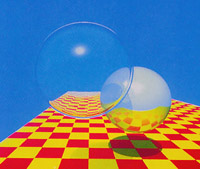
\includegraphics{early-raytracing-whitted}
    \centering
    \caption{Turner Whitted's original 1980 \cite{article:raytracing} image showing off the usage of ray tracing for
    reflection, refraction and shadows.}
    \label{fig:early-raytracing-whitted}
\end{figure}
Building upon ray tracing, an improved algorithm was published in 1986 by James T. Kajiya which used ray tracing
combined with a Monte Carlo algorithm in order to create a new algorithm that was called \emph{Monte
Carlo ray tracing} \cite{inproceedings:pathtracing}. Nowadays, Monte Carlo ray tracing is better
known as \emph{path tracing}.

It took another decade for path tracing to become the
physically based rendering approach that it is known for today. In 1996, Eric Lafortune improved
the algorithm by suggesting the usage of bidirectional path tracing \cite{techreport:pbr} and
finally the \ac{mlt} was suggested in 1997 by Eric Veach and Leonidas J. Guibas \cite{inproceedings:metropolis} to
improve performance in complex scenes.

This was the last notable improvement to the algorithm,
though many micro optimizations have since been published. All of these achievements and
improvements are generally collapsed into the term \emph{path tracing} since they do not diverge
from the general algorithm but instead improve upon it.

It took longer still for the industry to become interested in path tracing. The early interest in
ray tracing was of mostly academical and recreational nature. One of the most notable creations of
the early days of ray tracing is \emph{The Juggler} created and published by Eric Graham in 1986
\cite{site:juggler} on an Amiga 1000. It was a pre-rendered animation using ray tracing. Eric Graham
stated that it took the Amiga 1 hour to render each frame \cite{site:juggler}.

\begin{figure}[H]
    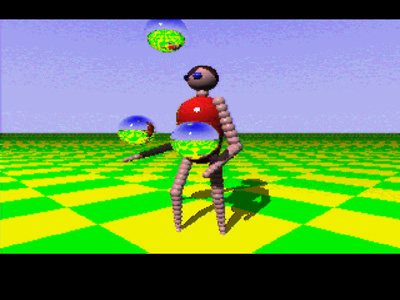
\includegraphics[scale=0.5]{amiga-juggler}
    \centering
    \caption{Eric Graham's Juggler}
    \label{fig:amiga-juggler}
\end{figure}
While the animation seems very primitive compared to the animations of today, it was exceptional at
the time. Ernie Wright's statement about his creation provides some contemporary context:

\blockquote[\cite{site:juggler}]{Turner Whitted's paper (1980) is widely regarded as the first modern
    description of ray tracing methods in computer graphics. This paper's famous image of balls floating
    above a checkerboard floor took 74 minutes to render on a DEC VAX 11/780 mainframe, a \$400,000
computer. The Juggler would appear a mere six years later, created and displayed on a \$2000 Amiga.}

The first feature-length computer-animated film,
\textit{Toy Story}, released in 1995 \cite{wiki:toy-story}, is sometimes miscredited as being the
first film using a ray tracing-like algorithm. However, it actually used traditional scanline
rendering. The first feature-length film using ray tracing, \textit{Cars}, was released much later,
in 2006 \cite{wiki:cars} \cite{inproceedings:cars} and started a wave of interest in the movie industry.

The first example of \emph{real time} path tracing was likely produced by the demo scene
\cite{wiki:demoscene} which was quick to adopt it \cite{site:realtime-radiosity-demos}
for the purpose of producing complex graphics rendered and generated on the fly. One notable
example of this is the WebGL Path Tracing by Evan Wallace made in 2010
\cite{site:webgl-path-tracing} which runs in most modern web browsers, making path tracing very
accessible.

\begin{figure}[H]
    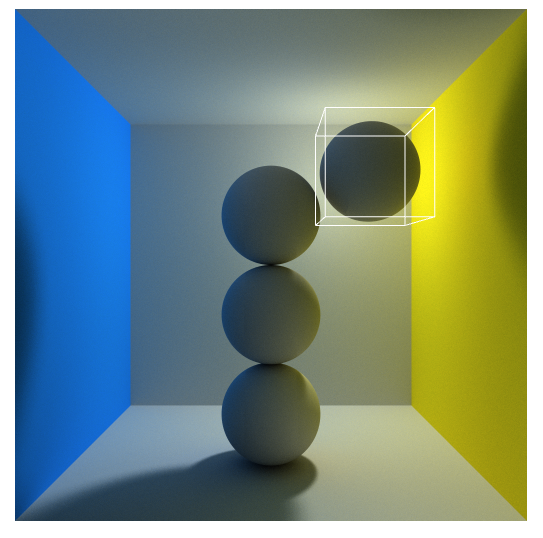
\includegraphics[scale=0.4]{webgl-pathtracer}
    \centering
    \caption{WebGL Path Tracer by Evan Wallace}
    \label{fig:webgl-pathtracer}
\end{figure}

Another example is the demo \textit{5 faces} by Fairlight from 2013
\cite{wiki:5faces-fairlight} which
uses a real time ray tracer running on the \acs{gpu} to render a complex scene at 30 \acs{fps}.

\begin{figure}[H]
    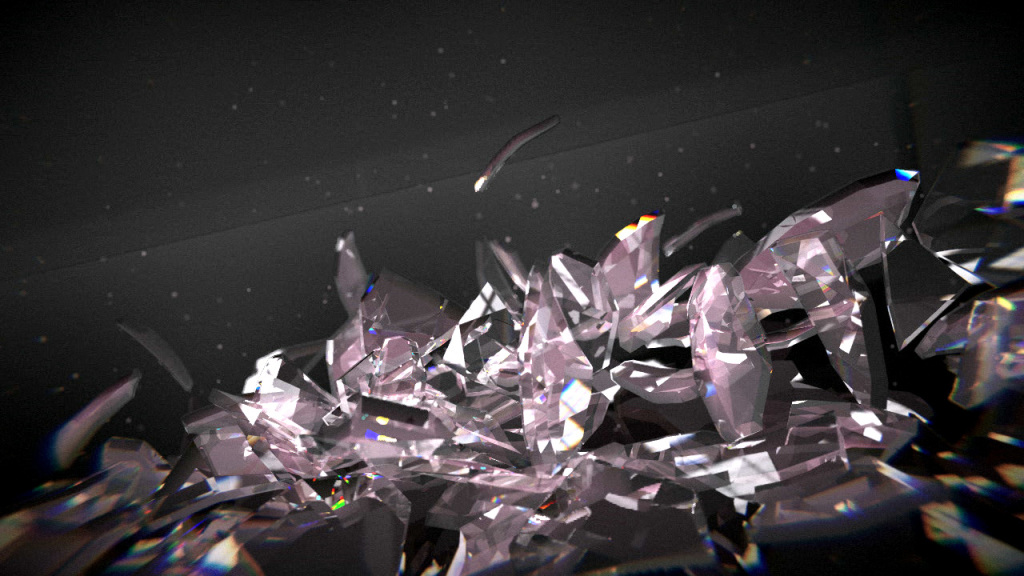
\includegraphics[scale=0.5]{5faces}
    \centering
    \caption{5 faces by Fairlight}
    \label{fig:5faces}
\end{figure}

In the past, some critics have offered critical insights about why it might not be a viable
alternative to rasterization on consumer hardware in the short term
\cite{site:raytracing-vs-rasterization} \cite{site:codinghorror-raytracing}. Even John Carmack of
id Software was sceptical of real time ray tracing in games in 2012 in a comment on Ars Technica
\cite{site:carmack-scepticism}.

\section{Current State of Technology}
Recent interest in real time path tracing is at peak levels. The most notable
example of this is Jacco Bikker's and Jeroen van Schijndel's \emph{Brigade Renderer} \cite{article:brigade}
\cite{site:brigade}. This renderer is aimed at game developers and is meant to run on commodity
hardware in real time. Its company, OTOY, is also developing a cloud-based rendering solution
called Octane Render \cite{site:octane} for animation professionals.

Microsoft's DirectX 12 \cite{site:dx12-raytracing} is receiving \emph{Hybrid Ray-Traced Shadows}, a
technology that combines real time ray tracing with rasterization to create fast high quality
shadows.

A video game using actual real time path tracing and physics called \emph{Sfera} was created by
David Bucciarelli \cite{site:sfera} in 2011. It uses OpenCL for calculating the paths and OpenGL to
render them to the screen.

It's important to keep in mind that while the real time graphics industry has mostly been driven by
video games, the most important hardware currently exist in game consoles which generally evolve at
a much slower pace than desktop computers in terms of hardware power and their graphics hardware
especially is usually non-upgradeable. This means that it wouldn't be economically viable to
develop a real time path tracing renderer that only ran on current generation desktop computers
because most consumers would not be able to benefit from the technology.

\chapter{Research}
The entirety of the practical research in this thesis was done with a Monte Carlo path tracer called
\emph{trac0r} \cite{site:trac0r}.
An effort was made to find an existing open source implementation of a path tracer focused on
real time applications but none seem to exist as of this writing. The most likely cause for that is
the enormous hardware cost currently still associated with doing real time path tracing.

\section{Implementation}
Alongside this thesis, a Monte Carlo path tracer called trac0r \cite{site:trac0r} was implemented in
C++14. It uses a library called glm \cite{site:glm} for linear algebra and most
other mathematical operations. Since trac0r itself is only a library, a graphical application making use
of it was implemented to showcase its results. This application is called \emph{trac0r\_viewer} and
uses SDL2 \cite{wiki:sdl} for input and output.\ trac0r\_viewer allows for interactive scene
navigation, visual debugging and automatic benchmarking.

A conscious decision was made to
only implement triangles for geometric primitives due to two reasons. Firstly, since every
other geometric shape can be expressed easily using an amount of triangles, it seems unnecessary to
add additional complexity (although using triangles to approximate other shapes will be less
efficient from a performance perspective). Secondly, real world applications very rarely make use of perfect
mathematical shapes such as spheres, boxes and tori when rendering. Most modern mesh modeling
approximates these shapes using triangles. Since this renderer is supposed to be used for real
world application such as games and interactive visualizations, it didn't seem necessary to
implement anything in addition to what mesh modeling tools will export. 

Additionally to triangles, \acp{aabb} were implemented with the aim to speed up rendering. While
trac0r does not implement any advanced acceleration structures (such as \acp{bvh} or kd-trees),
it uses \acp{aabb} to
dramatically decrease the number of triangle intersection tests. Every ray first tests for
intersections with every \ac{aabb} in the scene and upon a hit tests every triangle enclosed by the
\ac{aabb}. The fast Möller–Trumbore intersection algorithm \cite{inproceedings:moller2005fast} is used for
triangle intersection tests.

The program does not currently support importing of externally defined scenes or meshes. Scenes are
defined in-code. Methods for generating planes, boxes and icosahedra out of triangles are
provided. A properly sized \ac{aabb} is built around every shape.

It uses classic reverse path tracing and can optionally make use of OpenCL or OpenMP in order to
speed up computation.

\subsection{Design Overview}
When deciding to implement a path tracer, one first has to assemble a list of requirements and
components that go into creating it. Not all path tracers are built the same.

The list of requirements for trac0r before it was implemented ordered by descending priority is
provided below:

\begin{enumerate}
    \item \textbf{Speed}. In a real time path tracer, rendering speed is of utmost importance as one needs
        to target interactive frame rates at acceptable image quality. The trade-off here is that
        the image is allowed to be grainy as long as it can be shown to the user very quickly.
    \item \textbf{Ease of implementation}. Since the nature and scope of this thesis does not allow for implementing
        the most advanced algorithms, the only constraint for the implementation is for it to be
        good enough for benchmarking.
    \item \textbf{Interactivity}. The path tracer should show off basic interactivity. It should be
        noted, however, that it will probably not reach the requirements for \emph{real time}
        as lined out in chapter \ref{introduction} due to hardware constraints.
    \item \textbf{Portability}. The software should run on different GPUs as well CPUs with different
        memory and core configurations respectively with minimal effort. It should therefore be
        written with this portability in mind to make it easier to adapt.
    \item \textbf{Maintainability}. The software should be easy to understand, well-documented and
        easy to debug. Code should be commented where necessary.
\end{enumerate}

These requirements and priorities directed and
influenced many decisions and trade-offs made during the implementation.

The components that make up the path tracer follow:

\begin{description}
    \item[Random number generation] Solid and fast function for pseudo random number generation.
    \item[Camera] A structure that keeps all camera data as well as some functions to do coordinate
        transformations.
    \item[Material system] The path tracer should support four materials: Emitter, diffuse, glossy,
        glass. Each of them should at least provide their \ac{brdf}.
    \item[AABBs] A simple way to represent \acp{aabb}.
    \item[Triangles] The only kind of primitive that materials can be applied unto and in fact the
        only kind of geometry that is rendered.
    \item[Shapes and geometry] It should provide a way to generate basic geometric shapes. No
        mechanism for loading externally defined models is planned.
    \item[Scene] A way to efficiently save an arbitrary number of shapes. At first this should be
        implemented as a flat list. If there is enough time, a more efficient method should be
        considered.
    \item[Intersection/Scene lookup] Implemented as a ray intersection function for each supported primitive
        (which in this case means ray-AABB intersection and ray-triangle intersection).
    \item[Viewer] An interactive viewport that shows off progressive rendering with a sample scene.
\end{description}

These components are implemented in the following files:

\begin{table}[H]
    \centering
    \begin{tabularx}{\textwidth}{l | X}
        File(s)                    & Description \\ \hline
        trac0r/aabb.\{cpp,hpp\}      & \texttt{AABB} class implementation. \\
        trac0r/camera.\{cpp,hpp\}    & \texttt{Camera} class implementation with many helper methods. \\
        trac0r/flat\_structure.\{cpp,hpp\}  & Simple flat data structure implementation for scene geometry.
                                     Also contains the intersection logic for all contained
                                     geometry.\\
        trac0r/intersection\_info.hpp & Struct containing all relevant information about a single
                                     intersection. This struct is returned by all intersection
                                     methods. \\
        trac0r/intersections.hpp   & Contains functions for testing primitives for intersections. \\
        trac0r/material.hpp        & \texttt{Material} struct containing all material state. \\
        trac0r/random.hpp          & Implements functions to generate random floating point
                                     numbers, integers. Also contains functions for random
                                     geometric sampling with uniform and cosine-weighted
                                     distributions. \\
        trac0r/ray.hpp             & Contains the \texttt{Ray} struct which is used by every ray in
                                     trac0r.\\
        trac0r/renderer\_aux.cl    & OpenCL code containing the code for a single trace through the
                                     scene. Implements the BRDFs for all materials. \\
        trac0r/renderer\_aux.cpp   & C++ code containing the code for a single trace through the
                                     scene. Implements the BRDFs for all materials. \\
        trac0r/renderer.\{cpp,hpp\}  & Contains code for preparing the
                                     OpenCL and C++ renderer. \\
        trac0r/scene.\{cpp,hpp\}     & Simple \texttt{Scene} class serving as an abstract interface
                                     to the underlying data structure. \\
        trac0r/shape.\{cpp,hpp\}     & Contains a few factory methods for generating different kinds
                                     of geometry.\\
        trac0r/timer.hpp           & High-resolution timer for profiling purposes. \\
        trac0r/triangle.hpp        & A simple struct for expressing a
                                     triangle. \\
        trac0r/utils.hpp           & Contains various small helper functions for translating OpenCL
                                     error codes, packing packing and unpacking colors and
                                     displaying text.
    \end{tabularx}
    \caption{List of files in trac0r}
\end{table}

\subsection{Materials}
trac0r implements the following materials:
\begin{description}
    \item[Emitter] Arguably the most important material as it is the one providing the light to a
        scene. This simulates a black body heated to a certain temperature and as such serves as an
        area light when applied to geometry. Any ray hitting geometry using the emitter material is
        terminated. A scene without any geometry using emitter material will be utterly dark.
    \item[Diffuse] A matte material that scatters light to a random location on the hemisphere
        around the normal of the intersected geometry.
    \item[Glass] A material that will choose between reflection and refraction depending on the
        Fresnel coefficients \cite{wiki:fresnel}. It is the only material capable of handling
        intersections within an object.
    \item[Glossy] A metal-like material that will reflect a ray towards a cone centered around the
        direction of the outgoing light \(\omega_\text{o}\). A roughness parameter determines 
        the opening angle of that cone. A roughness of 0 will result in a perfect mirror while a roughness
        of 1 will produce a cone with an angle of \(\pi\).
\end{description}

\begin{minted}[linenos, autogobble]{c++}
    struct Material {
        /**
        * @brief Used to determine the material type used.
        * Refer to the table below:
        *        m_type = 1: Emissive
        *        m_type = 2: Diffuse
        *        m_type = 3: Glass
        *        m_type = 4: Glossy
        */
        uint8_t m_type = 1;

        /**
        * @brief Used as the basic color for most materials.
        */
        glm::vec3 m_color = {0.9f, 0.5f, 0.1f};

        /**
        * @brief Used to determine the ratio between reflection and diffusion
        * for some materials. Value must be between 0.0 and 1.0.
        */
        float m_roughness = 0.f;

        /**
        * @brief Index of refraction (IOR) is used to determine how
        * strongly light is bent inside a glass material.
        */
        float m_ior = 1.f;

        /**
        * @brief Luminous emittance provides the strength of emissive
        * material. Values can be larger than 1.0.
        */
        float m_emittance = 0.f;
    };
\end{minted}
\begingroup
\captionof{listing}{Material struct in trac0r\label{lst:trac0r-material}. Depending on the
\texttt{m\_type} set, different attributes of this material are used.}
\endgroup

\subsection{Shapes, Triangles and AABBs}

In trac0r, shapes are generators for a collection of triangles in a certain configuration. For
instance, a \texttt{plane} shape generates a list of two triangles that are configured in such a way
that they will form a quadratic flat surface with an orientation and scale as provided by the
constructor. In addition, shapes also take care of generating a well-fitting \ac{aabb}.

\begin{minted}[linenos, autogobble]{c++}
class Shape {
  public:
    static Shape make_box(glm::vec3 pos, glm::vec3 orientation,
                          glm::vec3 size, Material material);

    static Shape make_icosphere(glm::vec3 pos, glm::vec3 orientation,
                                float radius, size_t iterations,
                                Material material);

    static Shape make_plane(glm::vec3 pos, glm::vec3 orientation,
                            glm::vec2 size, Material material);

  protected:
    glm::vec3 m_pos;
    glm::vec3 m_orientation;
    glm::vec3 m_scale;
    AABB m_aabb;
    std::vector<Triangle> m_triangles;
};
\end{minted}
\begingroup
\captionof{listing}{Shape class in trac0r\label{lst:trac0r-shape}. The static methods serve as
factory functions.}
\endgroup

\vspace{1cm}

\acp{aabb} and triangles are rather simple:

\begin{minted}[linenos, autogobble]{c++}
    struct AABB {
        glm::vec3 m_min;
        glm::vec3 m_max;
    };
\end{minted}
\begingroup
\captionof{listing}{\ac{aabb} struct in trac0r\label{lst:trac0r-aabb}. Its extents are set by the
shape it is part of.}
\endgroup

\begin{minted}[linenos, autogobble]{c++}
    struct Triangle {
        glm::vec3 m_v1; // first vertex
        glm::vec3 m_v2; // second vertex
        glm::vec3 m_v3; // third vertex
        Material m_material;
        glm::vec3 m_normal;
        glm::vec3 m_centroid;
        float m_area;
    }:
\end{minted}
\begingroup
\captionof{listing}{Triangle struct in trac0r\label{lst:trac0r-triangle}. \texttt{m\_normal},
\texttt{m\_centroid} and \texttt{m\_area} are pre-calculated on construction.}
\endgroup

\subsection{Camera and Rays}

The camera is configured during the scene setup and sent to the \ac{gpu} every frame.

\begin{minted}[linenos, autogobble]{c++}
    class Camera {
        glm::vec3 m_pos;
        glm::vec3 m_dir;
        glm::vec3 m_world_up;
        glm::vec3 m_right;
        glm::vec3 m_up;
        float m_canvas_width;
        float m_canvas_height;
        glm::vec3 m_canvas_center_pos;
        glm::vec3 m_canvas_dir_x;
        glm::vec3 m_canvas_dir_y;
        float m_near_plane_dist;
        float m_far_plane_dist;
        int m_screen_width;
        int m_screen_height;
        float m_vertical_fov;
        float m_horizontal_fov;
    }
\end{minted}
\begingroup
\captionof{listing}{Camera class in trac0r. Implementation details are left out for the sake
of brevity. The reader should note, however, that many of the attributes shown here are
pre-calculated during construction and some are re-calculated every frame.}
\endgroup

\begin{minted}[linenos, autogobble]{c++}
    struct Ray {
        glm::vec3 m_origin;
        glm::vec3 m_dir;
        glm::vec3 m_invdir;
    };
\end{minted}
\begingroup
\captionof{listing}{Ray struct in trac0r. \texttt{m\_invdir} is pre-calculated upon construction.}
\endgroup

\subsection{Random Numbers}
Since the Monte Carlo method lives from random sampling, it needs a solid way of generating random
numbers. As it turns out, this is actually harder than one might think. While there are a great
many algorithms out there for getting random numbers, for the purposes of Monte Carlo integration
in a real time path tracing renderer, the right algorithm has to be chosen very carefully. The most
important requirement for this purpose is speed of generation. The C standard library comes with
\texttt{rand()} but sadly it's unusable for our purposes since it uses global state
shared by all threads which makes it effectively single threaded and therefore too slow.
The random generators in the C++ standard library provide good quality random numbers but are too
slow.

In fact, most random number generators are too slow when having to generate tens of millions of numbers per
second. Eventually, it was decided to use \texttt{xorshift}-type generators from Sebastiano Vigna
\cite{site:xorshift}. The \texttt{xorshift64star} generator is used to provide the seeds for the
\texttt{xorshift1024star} generator which is in turn used to generate the actual random numbers.
Additionally, the \texttt{xorshift1024star} generator is very efficient to use on \acp{gpu} due to
it not using any expensive operations such as divisions, \texttt{sqrt} or \texttt{pow}.

\begin{minted}[linenos, autogobble]{c++}
    inline uint64_t xorshift64star(uint64_t x) {
        x ^= x >> 12; // a
        x ^= x << 25; // b
        x ^= x >> 27; // c
        return x * 2685821657736338717LL;
    }
\end{minted}
\begingroup
\captionof{listing}{Function to quickly generate random numbers with a short period
\cite{site:xorshift}\label{lst:trac0r-xorshift64star}}
\endgroup

\begin{minted}[linenos, autogobble]{c++}
    inline int64_t xorshift1024star(uint64_t &p, std::array<uint64_t, 16> &s) {
    uint64_t s0 = s[p];
    uint64_t s1 = s[p = (p + 1) & 15];
    s1 ^= s1 << 31; // a
    s1 ^= s1 >> 11; // b
    s0 ^= s0 >> 30; // c
    return (s[p] = s0 ^ s1) * 1181783497276652981LL;
}
\end{minted}
\begingroup
\captionof{listing}{Function to quickly generate random numbers with a large period
\cite{site:xorshift}\label{lst:trac0r-xorshift1024star}}
\endgroup

\subsection{Sampling}
trac0r provides a few different methods for geometric sampling.

\begin{minted}[linenos, autogobble]{c++}
    /**
    * @brief Selects a random point on a sphere with uniform distribution.
    * point on a uniform.
    *
    * @return A random point on the surface of a sphere
    */
    inline glm::vec3 uniform_sample_sphere() {
        glm::vec3 rand_vec =
        glm::vec3(rand_range(-1.f, 1.f),
        rand_range(-1.f, 1.f),
        rand_range(-1.f, 1.f));
        return glm::normalize(rand_vec);
    }
\end{minted}
\begingroup
\captionof{listing}{Function to sample random points on the surface of a sphere implemented from
\cite{marsaglia1972choosing}\label{lst:trac0r-uniform-sampling}}
\endgroup  

\begin{minted}[linenos, autogobble]{c++}
    /**
    * @brief Given a direction vector, this will return a random uniform
    * point on a sphere on the hemisphere around dir.
    *
    * @param dir A vector that represents the hemisphere's center
    *
    * @return A random point the on the hemisphere
    */
    inline glm::vec3 oriented_uniform_hemisphere_sample(glm::vec3 dir) {
        glm::vec3 v = uniform_sample_sphere();
        return v * glm::sign(glm::dot(v, dir));
    }
\end{minted}
\begingroup
\captionof{listing}{Function to sample uniform points on a hemisphere given by
\texttt{dir}\label{lst:trac0r-oriented-uniform-sampling}}
\endgroup

\begin{minted}[linenos, autogobble]{c++}
    /**
    * @brief Selects a random point on a sphere with uniform or
    * cosine-weighted distribution.
    *
    * @param dir A vector around which the hemisphere will be centered
    * @param power 0.f means uniform distribution while 1.f means
    * cosine-weighted
    * @param angle When a full hemisphere is desired, use pi/2.
    * 0 equals perfect reflection. The value
    * should therefore be between 0 and pi/2. This angle is equal
    * to half the cone width.
    *
    * @return A random point on the surface of a sphere
    */
    inline glm::vec3 sample_hemisphere(glm::vec3 dir, float power, float angle) {
        glm::vec3 o1 = glm::normalize(ortho(dir));
        glm::vec3 o2 = glm::normalize(glm::cross(dir, o1));
        glm::vec2 r = glm::vec2{rand_range(0.f, 1.f),
        rand_range(glm::cos(angle), 1.f)};
        r.x = r.x * glm::two_pi<float>();
        r.y = glm::pow(r.y, 1.f / (power + 1.f));
        float oneminus = glm::sqrt(1.f - r.y * r.y);
        return glm::cos(r.x) * oneminus * o1 +
        glm::sin(r.x) * oneminus * o2 + r.y * dir;
    }
\end{minted}
\begingroup
\captionof{listing}{Function to sample cosine-weighted points on a hemisphere given by
    \texttt{dir}. \texttt{power} is used to determine whether to generate uniform samples or
    cosine-weighted ones. If \texttt{power} is \texttt{0.f}, uniform samples are generated. If it's
    \texttt{1.f}, cosine-weighted samples are generated. \texttt{angle} provides the opening angle of
    the cone that rays will be generated inside of.
    \label{lst:trac0r-hemisphere-sampling}
    \cite{site:better-sampling} \cite{site:cosine-weighted-hemisphere} \cite{site:path-tracing-3d-fractals}}
\endgroup

\begin{minted}[linenos, autogobble]{c++}
    /**
    * @brief Given a direction vector, this will return a random
    * cosine-weighted point on a sphere on the hemisphere around dir.
    *
    * @param dir A vector that represents the hemisphere's center
    *
    * @return A random point the on the hemisphere
    */
    inline glm::vec3 oriented_cosine_weighted_hemisphere_sample(glm::vec3 dir) {
        return sample_hemisphere(dir, 1.f, glm::half_pi<float>());
    }
\end{minted}
\begingroup
\captionof{listing}{Helper function to get samples from an entire hemisphere making use of
    the code in listing
\ref{lst:trac0r-hemisphere-sampling}\label{lst:trac0r-oriented-cosine-weighted-sampling}}
\endgroup

\begin{minted}[linenos, autogobble]{c++}
    /**
    * @brief Selects a random point on a cone with cosine-weighted
    * distribution.
    *
    * @param dir Direction in which the cone is oriented
    * @param angle Angle of the cone in radians
    *
    * @return A random point on the surface of a cone
    */
    inline glm::vec3 oriented_cosine_weighted_cone_sample(glm::vec3 dir,
    float angle) {
        return sample_hemisphere(dir, 1.f, angle);
    }
\end{minted}
\begingroup
\captionof{listing}{Helper function to get samples from a partial hemisphere making use of
    the code in listing
\ref{lst:trac0r-hemisphere-sampling}\label{lst:trac0r-oriented-cosine-weighted-sampling-sone}}
\endgroup

To achieve anti-aliasing, rays are randomly offset within a pixel which results in smoother borders
around shapes. This technique is free of additional computational cost with Monte Carlo integration.
In comparison, rasterization renderers typically require costly methods such as MSAA, FXAA, MLAA
and so on \cite{site:eurogamer-antialiasing} to achieve the same effect.

\subsection{Russian Roulette}
A technique called \emph{Russian roulette} \cite{caflisch1998monte} is used for determining when to terminate a ray. This
technique is commonly used in Monte Carlo path tracers for this purpose. It works by defining a
criterion that is checked against a random value for every ray before the ray is tested for
intersection with the scene. If the test is positive, the ray is terminated. Otherwise the ray
survives and the probability is multiplied with the ray's energy in order to keep the total energy
constant. This technique can be very useful if the criterion is carefully chosen to have a higher
chance of terminating rays with lower energy than those with higher energy. The reason for that is
that rays with lower energy add little new information to the image as compared to those with high
energy. 

In this path tracer, the termination criterion used depends on depth as opposed to ray energy
because a ray with a higher depth will also typically transfer less energy than one with a low
depth. The formula for the termination heuristic in trac0r is

\[\text{continuation\_probability} = 1 - \frac 1 {\text{max\_depth} - \text{depth}}.\]

In code, this is expressed as:

\begin{minted}[linenos, autogobble]{c++}
    float continuation_probability = 1.f - (1.f / (max_depth - depth));
    if (rand_range(0.f, 1.0f) >= continuation_probability) {
        break;
    }
\end{minted}
\begingroup
\captionof{listing}{Russian roulette in trac0r \label{lst:trac0r-russian-roulette}}
\endgroup

\subsection{Scene Setup}
The scene is hardcoded in the \texttt{setup\_scene} method of trac0r\_viewer. The basic scene setup
follows these steps:

\begin{enumerate}
    \item Set up materials
    \item Set up shapes
    \item Add shapes to scene
    \item Set up camera
\end{enumerate}

The code listed below in~\ref{lst:trac0r-scene-setup} creates a basic test scene showing off all of
trac0r current materials and shapes. The basic setup resembles that the classic Cornell box. It has
a red diffuse left wall, a green diffuse right wall, white floor, white back wall and white ceiling.
A glossy box is placed inside the left half of the room while a white diffuse box is placed on the
right half of it. A icosahedron with a glass material is placed in its center in front of the
boxes. A glossy icosahedron is placed on top of the right box. A box with the emitter material is
placed under the ceiling to serve as a light. An almost fully converged picture of this scene can
be seen in figure~\ref{fig:trac0r-5000}.

In order to understand the code below refer to the Material listing~\ref{lst:trac0r-material}.

\begin{minted}[linenos, autogobble]{c++}
    void Viewer::setup_scene() {
        trac0r::Material emissive{1, {1.f, 0.93f, 0.85f}, 0.f, 1.f, 15.f};
        trac0r::Material default_material{2, {0.740063, 0.742313, 0.733934}};
        trac0r::Material diffuse_red{2, {0.366046, 0.0371827, 0.0416385}};
        trac0r::Material diffuse_green{2, {0.162928, 0.408903, 0.0833759}};
        trac0r::Material glass{3, {0.5f, 0.5f, 0.9f}, 0.0f, 1.51714f};
        trac0r::Material glossy{4, {1.f, 1.f, 1.f}, 0.09f};

        auto wall_left = trac0r::Shape::make_plane({-0.5f, 0.4f, 0},
                                    {0, 0, -glm::half_pi<float>()},
                                    {1, 1}, diffuse_red);
        auto wall_right = trac0r::Shape::make_plane({0.5f, 0.4f, 0},
                                    {0, 0, glm::half_pi<float>()},
                                    {1, 1}, diffuse_green);
        auto wall_back = trac0r::Shape::make_plane({0, 0.4f, 0.5},
                                    {-glm::half_pi<float>(), 0, 0},
                                    {1, 1}, default_material);
        auto wall_top = trac0r::Shape::make_plane({0, 0.9f, 0},
                                    {glm::pi<float>(), 0, 0},
                                    {1, 1}, default_material);
        auto wall_bottom = trac0r::Shape::make_plane({0, -0.1f, 0},
                                    {0, 0, 0},
                                    {1, 1}, default_material);
        auto lamp = trac0r::Shape::make_plane({0, 0.85f, -0.1},
                                    {0, 0, 0}, {0.4, 0.4}, emissive);
        auto box1 = trac0r::Shape::make_box({0.3f, 0.1f, 0.1f},
                                    {0, 0.6f, 0}, {0.2f, 0.5f, 0.2f},
                                    default_material);
        auto box2 = trac0r::Shape::make_box({-0.2f, 0.15f, 0.1f},
                                    {0, -0.5f, 0},
                                    {0.3f, 0.6f, 0.3f}, glossy);
        auto sphere1 = trac0r::Shape::make_icosphere({0.f, 0.1f, -0.3f},
                                    {0, 0, 0}, 0.15f, 2, glass);
        auto sphere2 = trac0r::Shape::make_icosphere({0.3f, 0.45f, 0.1f},
                                    {0, 0, 0}, 0.15f, 2, glossy);

        Scene::add_shape(m_scene, wall_left);
        Scene::add_shape(m_scene, wall_right);
        Scene::add_shape(m_scene, wall_back);
        Scene::add_shape(m_scene, wall_top);
        Scene::add_shape(m_scene, wall_bottom);
        Scene::add_shape(m_scene, lamp); 
        Scene::add_shape(m_scene, box1);
        Scene::add_shape(m_scene, box2);
        Scene::add_shape(m_scene, sphere1);
        Scene::add_shape(m_scene, sphere2);

        glm::vec3 cam_pos = {0, 0.31, -1.2};
        glm::vec3 cam_dir = {0, 0, 1};
        glm::vec3 world_up = {0, 1, 0};

        m_camera = Camera(cam_pos, cam_dir, world_up, 90.f, 0.001, 100.f,
        m_screen_width, m_screen_height);
    }
\end{minted} 
\begingroup
\captionof{listing}{Scene setup in trac0r\_viewer \label{lst:trac0r-scene-setup}}
\endgroup

\subsection{Tracing a Ray}
trac0r roughly follows the algorithm outlined in \ref{algorithm}.

\begin{minted}[linenos, autogobble]{c++}
    // For every horizontal pixel
    for (uint32_t x = 0; x < m_width; x += stride_x) {
        // For every vertical pixel
        for (uint32_t y = 0; y < m_height; y += stride_y) {
            // Make a ray out of this pixel
            Ray ray = Camera::pixel_to_ray(m_camera, x, y);

            // Trace this new ray and save the color
            glm::vec4 new_color = trace_camera_ray(ray, max_depth);

            // Accumulate result into buffer
            m_luminance[y * m_width + x] = new_color;
        }
    }
\end{minted} 
\begingroup
\captionof{listing}{First, make a ray for every pixel, then trace it, finally accumulate the result into a buffer}
\endgroup

\begin{minted}[linenos, autogobble]{c++}
    IntersectionInfo intersect(const FlatStructure &flatstruct, const Ray &ray) {
        IntersectionInfo intersect_info;

        // Keep track of closest triangle
        float closest_dist = std::numeric_limits<float>::max();
        Triangle closest_triangle;
        for (const auto &shape : FlatStructure::shapes(flatstruct)) {
            if (intersect_ray_aabb(ray, Shape::aabb(shape))) {
                for (auto &tri : Shape::triangles(shape)) {
                    float dist_to_intersect;
                    bool intersected = 
                        intersect_ray_triangle(ray, tri, dist_to_intersect);
                    if (intersected) {
                        // Find closest triangle
                        if (dist_to_intersect < closest_dist) {
                            closest_dist = dist_to_intersect;
                            closest_triangle = tri;

                            intersect_info.m_has_intersected = true;
                            intersect_info.m_pos =
                                ray.m_origin + ray.m_dir * closest_dist;
                            intersect_info.m_incoming_ray = ray;

                            intersect_info.m_angle_between =
                                glm::dot(closest_triangle.m_normal,
                                         intersect_info.m_incoming_ray.m_dir);

                            intersect_info.m_normal =
                                closest_triangle.m_normal;
                            intersect_info.m_material =
                                closest_triangle.m_material;
                        }
                    }
                }
            }
        }

        return intersect_info;
    }
\end{minted} 
\begingroup
\captionof{listing}{Scene intersection routine}
\endgroup

\begin{minted}[linenos, autogobble]{c++}
    glm::vec4 Renderer::trace_camera_ray(const Ray &ray,
                                         const unsigned max_depth,
                                         const Scene &scene) {
        Ray next_ray = ray;
        glm::vec3 return_color{0.f};
        glm::vec3 luminance{1.f};
        size_t depth = 0;

        // We'll run until terminated by Russian Roulette
        while (true) {
            // Russian Roulette here as defined above
            depth++;

            auto intersect_info = Scene::intersect(scene, next_ray);
            if (intersect_info.m_has_intersected) {
                // Emitter Material
                if (intersect_info.m_material.m_type == 1) {
                    return_color =
                        luminance *
                        intersect_info.m_material.m_color *
                        intersect_info.m_material.m_emittance /
                        continuation_probability;
                    break;
                }

                // Diffuse Material
                else if (intersect_info.m_material.m_type == 2) {
                    // Find normal in correct direction
                    intersect_info.m_normal =
                        intersect_info.m_normal *
                        -glm::sign(intersect_info.m_angle_between);
                    intersect_info.m_angle_between =
                        intersect_info.m_angle_between *
                        -glm::sign(intersect_info.m_angle_between);

                    // Find new random direction for diffuse reflection

                    // We're using importance sampling for this since it
                    // converges much faster than uniform sampling
                    glm::vec3 new_ray_dir =
                        oriented_cosine_weighted_hemisphere_sample(
                            intersect_info.m_normal);
                    luminance *= intersect_info.m_material.m_color;

                    // Make a new ray
                    next_ray = Ray{intersect_info.m_pos, new_ray_dir};
                }

                // Glass Material
                else if (intersect_info.m_material.m_type == 3) {
                    // BRDF Omitted for brevity
                }

                // Glossy Material
                else if (intersect_info.m_material.m_type == 4) {
                    // BRDF Omitted for brevity
                }
            } else {
                break;
            }
        }

        return glm::vec4(return_color, 1.f);
    }
\end{minted} 
\begingroup
\captionof{listing}{Material state machine \cite{site:path-tracing-3d-fractals}}
\endgroup

\section{Results}
\subsection{Visual Results}
\begin{figure}[H]
    \subfloat[\(n = 1\)]{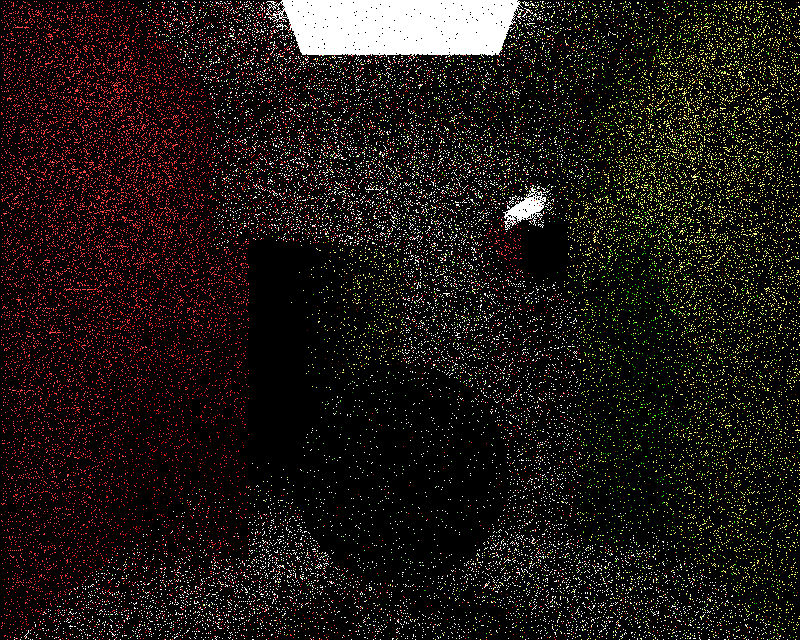
\includegraphics[scale=0.15]{trac0r-1.png}}
    \subfloat[\(n = 2\)]{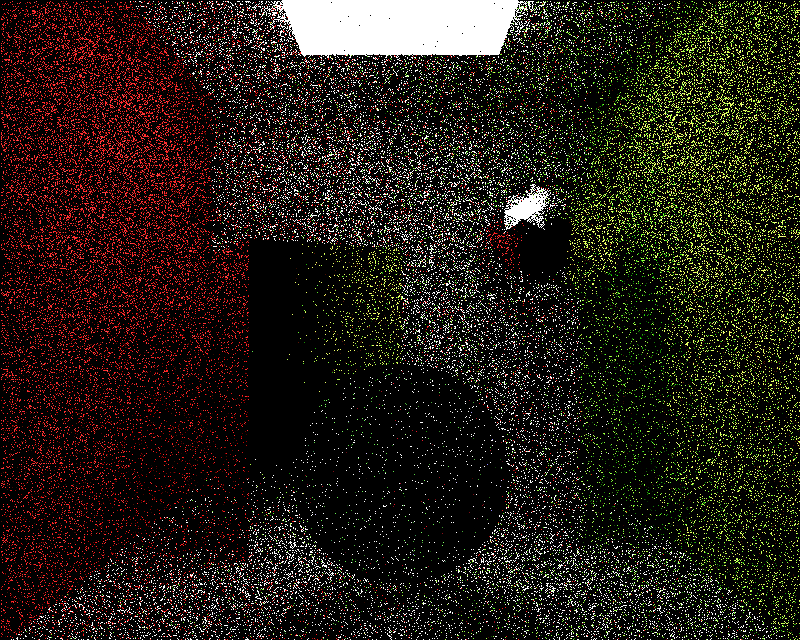
\includegraphics[scale=0.15]{trac0r-2.png}}
    \subfloat[\(n = 3\)]{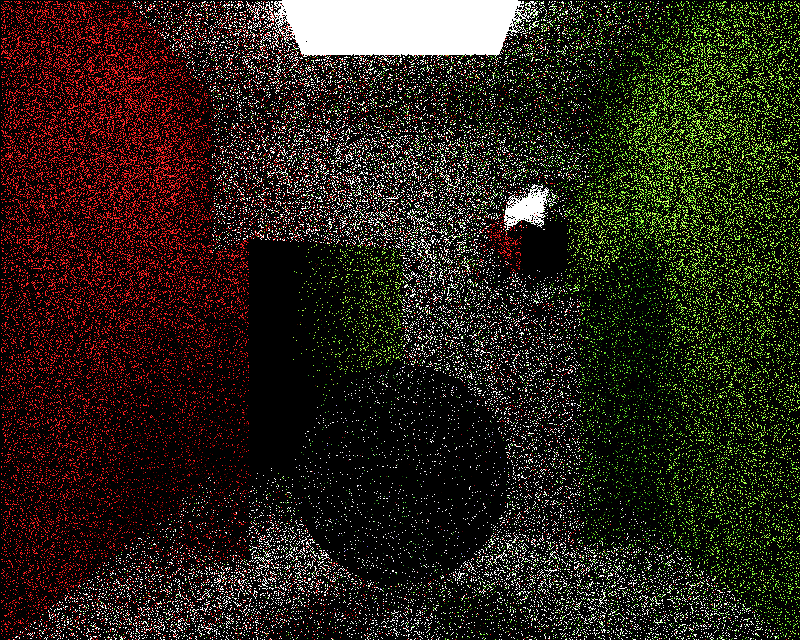
\includegraphics[scale=0.15]{trac0r-3.png}}
    \centering

    \subfloat[\(n = 4\)]{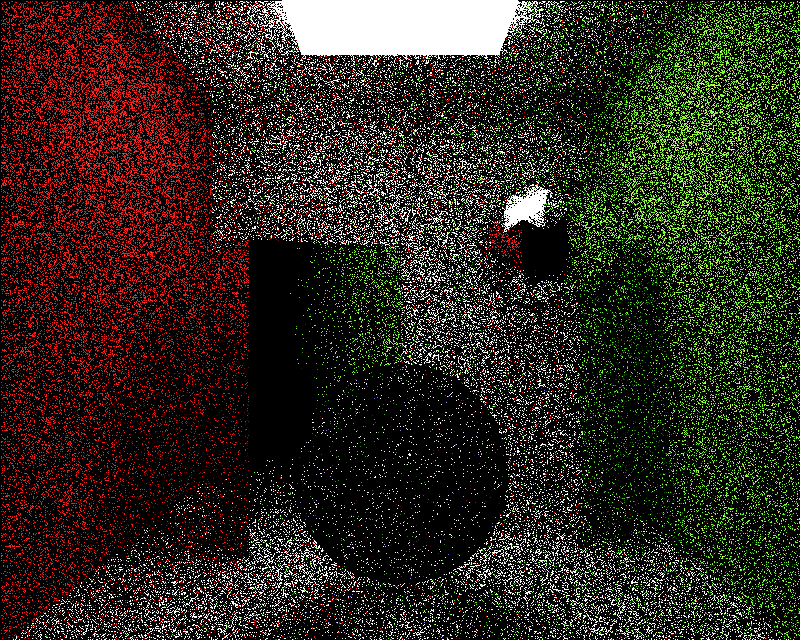
\includegraphics[scale=0.15]{trac0r-4.png}}
    \subfloat[\(n = 5\)]{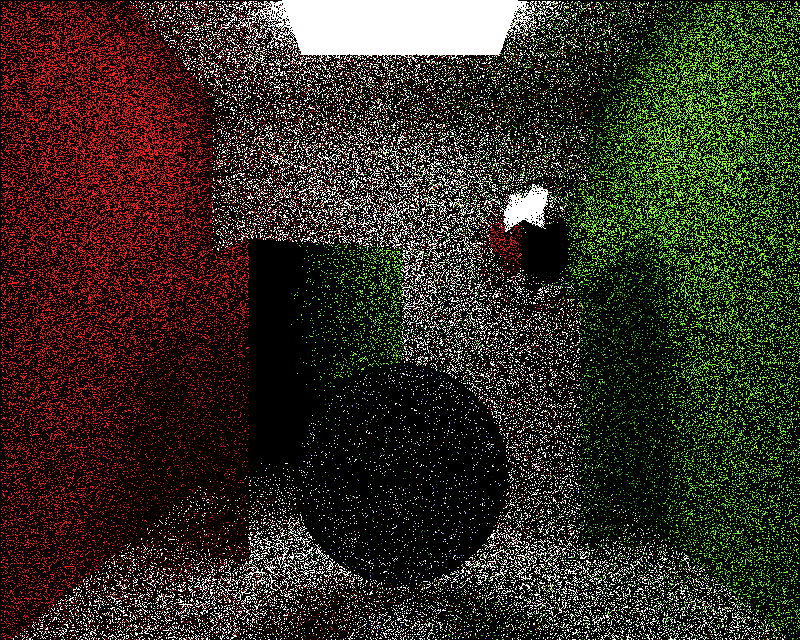
\includegraphics[scale=0.15]{trac0r-5.png}}
    \subfloat[\(n = 10\)]{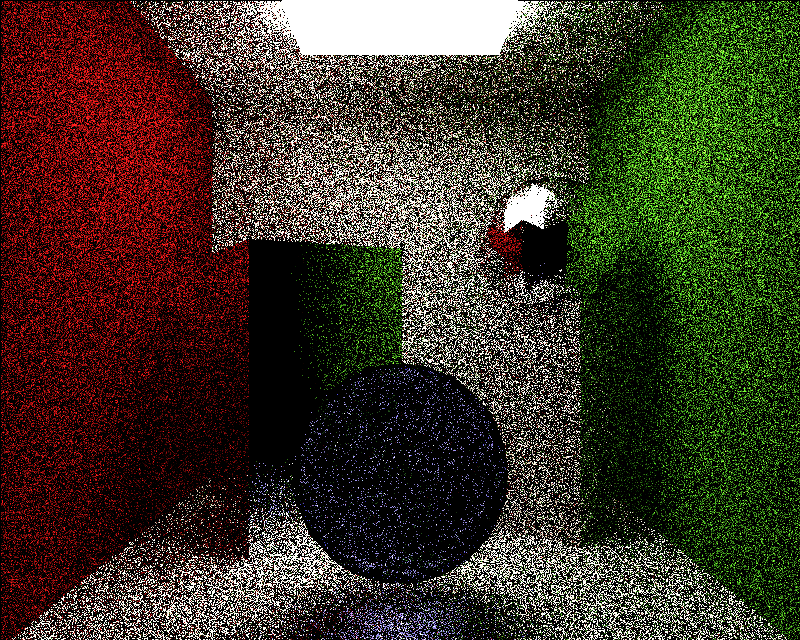
\includegraphics[scale=0.15]{trac0r-10.png}}
    \centering

    \subfloat[\(n = 20\)]{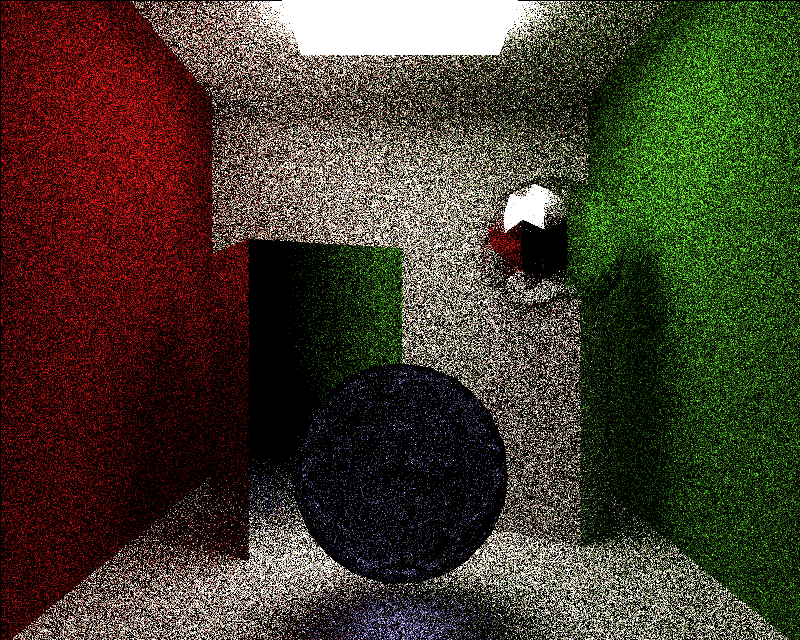
\includegraphics[scale=0.15]{trac0r-20.png}}
    \subfloat[\(n = 50\)]{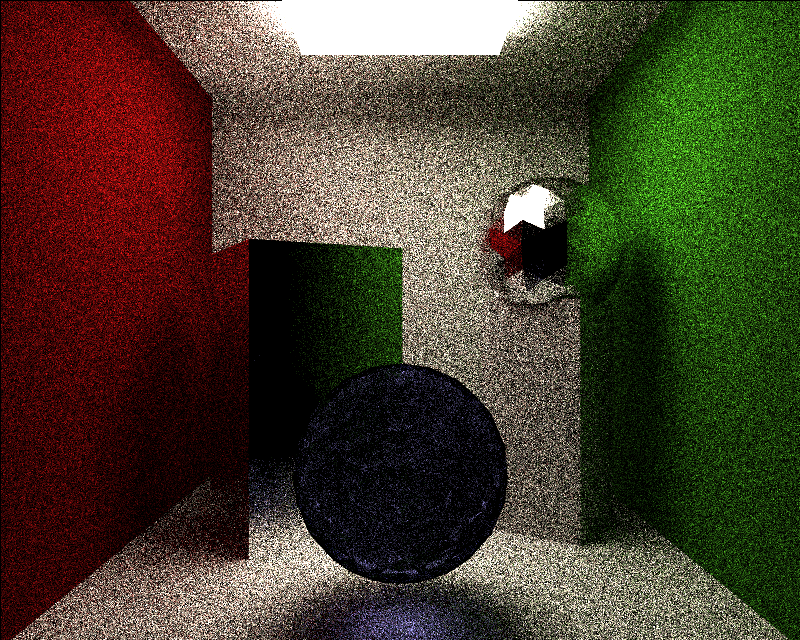
\includegraphics[scale=0.15]{trac0r-50.png}\label{fig:trac0r-50}}
    \subfloat[\(n = 100\)]{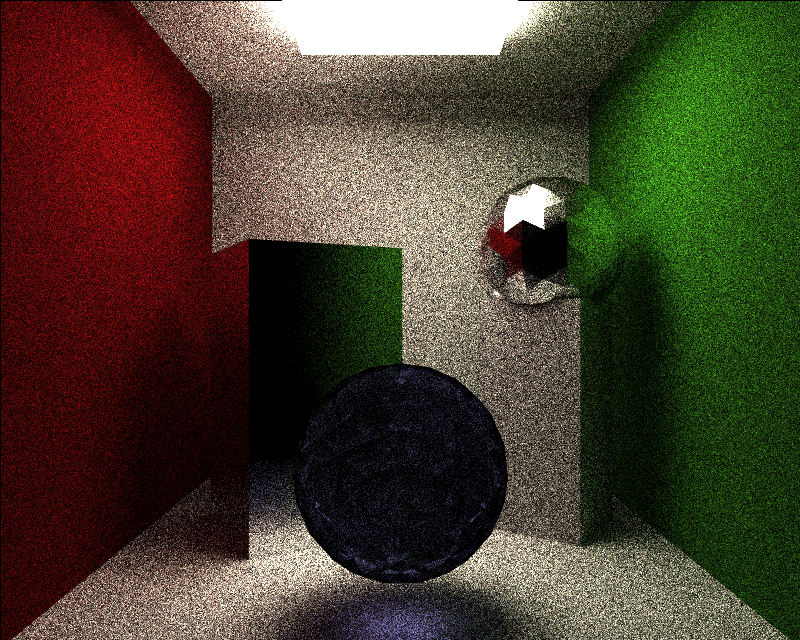
\includegraphics[scale=0.15]{trac0r-100.png}\label{fig:trac0r-100}}
    \centering
    \caption{trac0r\_viewer viewport after integrating \(n\) frames}
    \label{fig:trac0r_n_frames}
\end{figure}

While certainly subjective, frame~\ref{fig:trac0r-50} and~\ref{fig:trac0r-100} begin to start looking
acceptable. It took an average of 10 seconds to approach this kind of acceptable quality at a
resolution of 800x640 on an NVIDIA Geforce GTX 570.

\begin{figure}[H]
    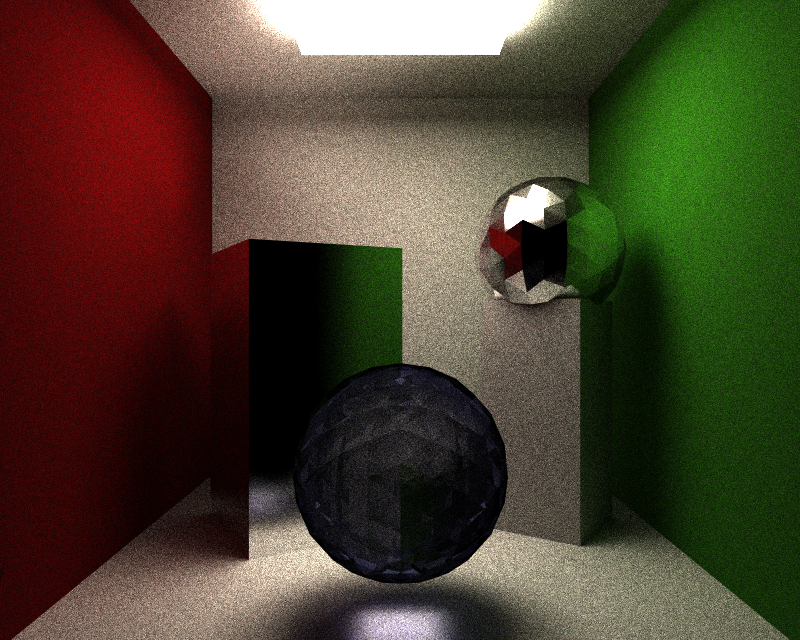
\includegraphics[scale=0.5]{trac0r-5000.png}
    \centering
    \caption{trac0r\_viewer after integrating for 5000 frames}
    \label{fig:trac0r-5000}
\end{figure}

The image shown in~\ref{fig:trac0r-5000} displays an almost fully converged image. It took almost 5
minutes to converge to this quality given the same parameters and hardware as above. The scene
shown here is described by the code given in listing~\ref{lst:trac0r-scene-setup}.

\subsection{Debug View}
\begin{figure}[H]
    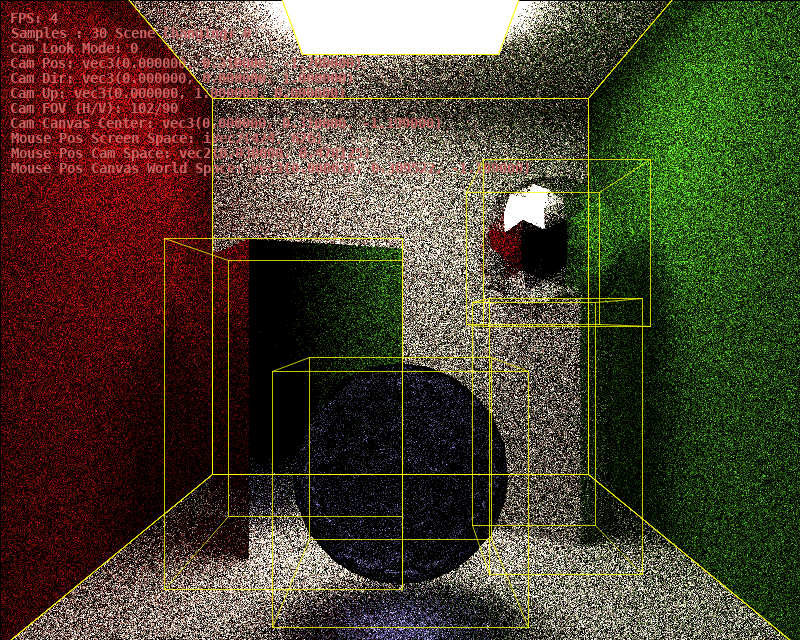
\includegraphics[scale=0.5]{trac0r-debug1.png}
    \centering
    \caption{trac0r\_viewer debug view}
    \label{fig:trac0r_debug1}
\end{figure}

Figure~\ref{fig:trac0r_debug1} above shows the debug view that can dynamically toggled during
runtime. It displays information about the current state of the camera as well as mouse position
and other helpful text in the upper left corner of the
viewport. The yellow boxes display the \acp{aabb} around the shapes because they are usually not
directly visible. This comes in handy when debugging visibility problems.

\begin{figure}[H]
    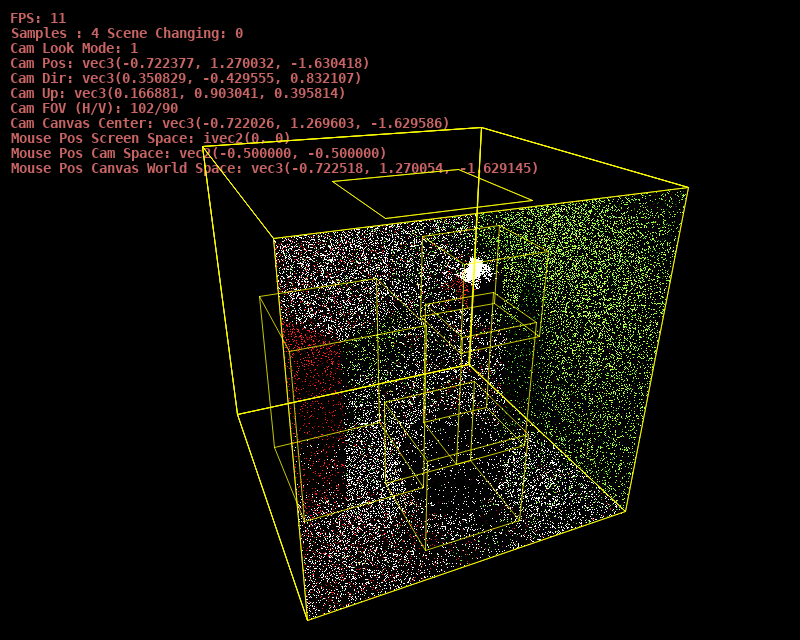
\includegraphics[scale=0.5]{trac0r-debug2.png}
    \centering
    \caption{trac0r\_viewer debug view while interactively navigating the scene}
    \label{fig:trac0r_debug2}
\end{figure}

As shown in figure~\ref{fig:trac0r_debug2}, trac0r\_viewer can be interactively navigated with
keyboard and mouse controls to control the camera in the scene. Upon every interaction, the scene
rendering begins accumulating samples anew. While the debug view is not necessary for
interactivity, it is activated in the image of~\ref{fig:trac0r_debug2} to better show the
transformation.

\subsection{Performance Results}
In order to be able to compare performance, an objective and reliable method and unit of
measure for doing so has to be decided upon. If this were a rasterizing renderer, \ac{fps} would be
an easy choice.
However, comparing \ac{fps} is not a particularly good criterion between different path tracers since
generally \ac{fps} doesn't correlate to rate of convergence. That is, one path tracer might be able
to iterate at 60 \ac{fps} but takes three seconds to converge while a different path tracer may
only be able to do 10 \ac{fps} but takes only 2 seconds to converge. This might seem unintuitive at
first but remember that path tracing is a very different algorithm compared to rasterization. In
rasterization, once a frame is rendered, the image is \emph{done}. It won't improve by rendering the
same scene a second time. In path tracing, particularly Monte Carlo path tracing, an image will be
improved with every new frame that is rendered using the same parameters due to how Monte Carlo
integration works.

In spite of that, this thesis uses \ac{fps} as the primary criterion for two reasons. Firstly, we are not
comparing different path tracers to the one made as part of the thesis. We only compare it
against itself in different scene and hardware configurations. Secondly, \ac{fps} is much easier
to work with and compare than image quality. One might use \ac{psnr} to do the latter but that
still leaves open the question of when to measure the image as even a single frame might take
longer than a second to render under specific circumstances.

\begin{minipage}{\textwidth}
    \begin{figure}[H]
        \begin{tikzpicture}
            \begin{axis}[
                    title={Performance in correlation to scene complexity},
                    xlabel={Triangles},
                    ylabel={FPS},
                    legend pos=north east,
                    ymajorgrids=true,
                    grid style=loosely dashed,
                    smooth,
                    cycle list name=exotic,
                    x tick label style={align=center, rotate=45},
                    width=\textwidth
                ]

                \addplot
                    coordinates {
                        (56,16.9)
                        (116,13.9)
                        (356,7.4)
                        (1316,2.6)
                        (5156,0.72)
                    };

                \addplot
                    coordinates {
                        (56,26)
                        (116,19.5)
                        (356,8.9)
                        (1316,2.8)
                        (5156,0.73)
                    };

                \addplot
                    coordinates {
                        (56,17.6)
                        (116,15.6)
                        (356,9.5)
                        (1316,3.7)
                        (5156,1.0)
                    };

                \addplot
                    coordinates {
                        (56,24)
                        (116,21.8)
                        (356,14)
                        (1316,5.8)
                        (5156,1.7)
                    };

                \addplot
                    coordinates {
                        (56,24)
                        (116,22.4)
                        (356,15)
                        (1316,6.2)
                        (5156,1.83)
                    };
                \legend{NVIDIA Geforce GTX 660, NVIDIA Geforce GTX 570,
                    NVIDIA Geforce GTX 960, NVIDIA Geforce GTX 970,
                NVIDIA Geforce GTX 980}
            \end{axis}
        \end{tikzpicture}
        \centering
        \caption{Scene complexity benchmark on a variety of graphics cards. It was benchmarked at
        a resolution of 800x600.}
        \label{fig:benchmark-scene-complexity}
    \end{figure}

    \begin{table}[H]
        \centering
        \begin{tabular}{l | r | r}
            GPU                     & Average FPS   & GFLOPS \\ \hline
            NVIDIA Geforce GTX 660  & 8.3           & 1881.6 \\
            NVIDIA Geforce GTX 570  & 11.6          & 1405.4 \\
            NVIDIA Geforce GTX 960  & 9.5           & 2308   \\
            NVIDIA Geforce GTX 970  & 13.5          & 3494   \\
            NVIDIA Geforce GTX 980  & 13.9          & 4612
        \end{tabular}
        \caption{Tested GPU performance and GFLOPS}
        \label{tbl:benchmark-table}
    \end{table}
\end{minipage}

Figure~\ref{fig:benchmark-scene-complexity} shows how \ac{fps} behaves in regards to triangle
count while table~\ref{tbl:benchmark-table} shows average \ac{fps} per \ac{gpu} as well as their
rated peak single-precision performance in \ac{gflops}.

We can see that the program performs quite poorly as triangle count is increased even at a
fairly low number of triangles as predicted with formula~\ref{eq:complexity} and in
table~\ref{tbl:triangle-intersections-count}.

It is also interesting to see that the difference in performance among the \acp{gpu} isn't nearly
as dramatic as their rated peak \ac{gflops} would suggest. This observation suggests that the
application is heavily memory bound.

\section{Evaluation}
In order to properly rate the results seen above and in figure \ref{fig:benchmark-scene-complexity},
they need to be put into perspective. Performance
of \acp{cpu} and \acp{gpu} varies enormously depending on their year of release due to technical
progress.

\begin{figure}[H]
    \begin{tikzpicture}
        \begin{axis}[
                title={GFLOPS of highend consumer desktop GPUs by year},
                xlabel={Year of release},
                ylabel={Peak single precision performance [GFLOPS]},
                xmin=2005,
                xmax=2020,
                ymin=0,
                ymode=log,
                log ticks with fixed point,
                legend pos=north west,
                ymajorgrids=true,
                xmajorgrids=true,
                legend cell align=left,
                grid style=loosely dashed,
                extra y ticks={500, 2500, 5000, 20000, 40000},
                x label style={below=5mm},
                extra y tick style={log identify minor tick positions=false},
                x tick label style={align=center, rotate=45, /pgf/number format/1000 sep={}},
                width=\textwidth
            ]

            \addplot+[
                    green!60!black,
                    only marks,
                    mark options={green!60!black},
                    point meta=explicit symbolic,
                    nodes near coords
                ]
                coordinates {
                    (2006,518) [\tiny Geforce 8800 GTX]
                    (2008,648) [\tiny Geforce 9800 GTX]
                    (2008,933) [\tiny Geforce GTX 280]
                    (2010,1345) [\tiny Geforce GTX 480]
                    (2010,1581) [\tiny Geforce GTX 580]
                    (2012,3090) [\tiny Geforce GTX 680]
                    (2013,3977) [\tiny Geforce GTX 780]
                    (2014,4612) [\tiny Geforce GTX 980]
                };

            \addplot+[
                    red,
                    only marks,
                    mark options={red},
                    point meta=explicit symbolic,
                    nodes near coords
                ]
                coordinates {
                    (2007,384) [\tiny Radeon HD 2900 PRO]
                    (2008,1200) [\tiny Radeon HD 4870]
                    (2009,2720) [\tiny Radeon HD 5870]
                    (2011,2703) [\tiny Radeon HD 6970]
                    (2012,3789) [\tiny Radeon HD 7970]
                    (2013,4849) [\tiny Radeon R9 290]
                    (2015,7168) [\tiny Radeon R9 Fury]
                };

            \addplot+[
                    gray,
                    smooth,
                    mark=none,
                    densely dashed,
                    thick
                ]
                coordinates {
                    (2004,250*0.7)
                    (2006,500*0.7)
                    (2008,1000*0.7)
                    (2010,2000*0.7)
                    (2012,4000*0.7)
                    (2014,8000*0.7)
                    (2016,16000*0.7)
                    (2018,32000*0.7)
                    (2020,64000*0.7)
                };
                % Formula is: 250*2^(0.5(x-2004))*0.7 x is from 2004 to 2020

            \legend{NVIDIA GPUs, AMD GPUs, Mean GFLOPS}
        \end{axis}
    \end{tikzpicture}
    \centering
    \caption{Mid-highend GPUs by year vs theoretical single-precision GFLOPS.
    All \ac{gflops} numbers are taken from the chip designers' official sites.}
    \label{fig:gpus-by-year}
\end{figure}

The logarithmic graph in figure~\ref{fig:gpus-by-year} shows the exponential growth of \ac{gflops} since 2004
when \acp{gpu} had approximately 250 \ac{gflops} of single-precision performance at their disposal.
The exponential function of the graph
(where \(x\) is an integer expressing the respective year) is
\[ f(x) = 250 * 2 ^ {0.5 (x-2004)} * 0.7 \]
and can be used to extrapolate \ac{gpu} performance until 2020 assuming the growth stays constant.
Following that assumption, there will be a \ac{gpu} capable of 10000 \ac{gflops} in 2016, 20000
\ac{gflops} in 2018 and 40000 \ac{gflops} in 2020.

It should be noted that while \ac{gflops} isn't the only relevant criterion to estimating the
performance of a \ac{gpu}, it's likely the most important one.

On the other hand, memory performance didn't keep up with floating point performance and therefore
the performance gap between memory and floating point speed widened. This has turned memory latency
and memory bandwidth into the most common bottleneck for modern \ac{gpu} applications.

Although certainly interesting, no graph for memory performance was created because
it is much harder to express in a single number since it's usually
a multi-tiered memory architecture where each tier has very different sizes
and performance characteristics and it also doesn't scale as predictably.

\chapter{Conclusion and Outlook}
The study set out to explore the question of when real time path tracing would become
a viable alternative to rasterization on consumer-level desktop hardware. It did so by defining
performance criteria that were chosen to be considered the minimum threshold for real time path tracing.
According to the criteria, real time path tracing would be achieved when a sufficiently converged
frame can be rendered within \(16.67ms\) (which works out to 60 \ac{fps}). The author realizes that
image quality is subjective but makes an attempt to be critical about quality.

A Monte Carlo path tracer was implemented as part of the study and is used to benchmark a selection
of current and past graphics hardware to extrapolate from. The path tracer was found to be heavily
memory bound as the speedup from using a \ac{gpu} with a better single-precision floating
point performance didn't match expectations. Additionally, the path tracer's implementation is
mostly naive and therefore doesn't match the current state of the art in terms of algorithmic
performance. As such, the benchmark results gained from this path tracer will be used as a lower
bound for expected performance.

The study also extrapolates graphics hardware performance by single-precision \ac{gflops} over the
course of 16 years. It was found that \ac{gpu} performance follows an exponential function and is
expected to continue in this manner. Extrapolating the data, single \acp{gpu} are expected to reach up to
40 TFLOPS by 2020.

Ongoing research in path tracing and related topics is likely to yield better better algorithms and
methods as
it has in the past. This is especially true for algorithms specifically meant to run on \acp{gpu}
as this is still a new topic that has yet to be explored in-depth.

While it is certainly hard to estimate when exactly real time path tracing will be viable, a
combination of modern methods for speeding up image convergence is likely to provide satisfactory
performance even today on more expensive hardware. The most important improvement over a naive
implementation of a path tracer
is most certainly found in employing a tree-based acceleration data structure such as a BVH or kd-tree.
This decreases
lookup time from \(O(n)\) to just \(O(\log(n)\) per ray. This would yield an effective speedup of
one to two orders of magnitude depending on scene complexity.
Convergence performance could best be improved by making use of bidirectional path tracing and
better sampling techniques such as \textit{Multiple Importance Sampling}. For scenes that are lit
mostly by indirect light, these techniques would lead to faster convergence by about a magnitude.

Apart from algorithmic improvements, the implementation's usage of \ac{gpu} memory architecture
is likely far from optimal and could be improved. \ac{gpu} memory speeds suggest that this would
lead to a general speedup around factor 5.

Lastly, overall image quality could be improved by running an image filter over the rendered image
before displaying it to the user. A suitable image filtering algorithm should be non-linear and
edge-preserving as well as energy-preserving so that it won't lower the quality of the resulting
image. A notable filter fulfilling those requirements is the \textit{bilateral filter}. This could
be used to display an image before it is fully converged. This is obviously a trade-off of quality
for performance but for the sake of speed it might be worth it.

All in all, the research suggests that real time path tracing could be a viable alternative to
rasterization in four years on upper level commodity hardware.
\listoffigures
\listoflistings
\listoftables
\bibliography{main}
\bibliographystyle{unsrt}

\chapter*{Eidesstattliche Erklärung}
\onehalfspace
„Hiermit versichere ich an Eides statt, dass ich die vorliegende Arbeit im
Studiengang Informatik selbstständig verfasst und keine anderen als die
angegebenen Hilfsmittel – insbesondere keine im Quellenverzeichnis nicht
benannten Internet-Quellen – benutzt habe. Alle Stellen, die wörtlich oder
sinngemäß aus Veröffentlichungen entnommen wurden, sind als solche kenntlich
gemacht. Ich versichere weiterhin, dass ich die Arbeit vorher nicht in einem
anderen Prüfungsverfahren eingereicht habe und die eingereichte schriftliche
Fassung der auf dem elektronischen Speichermedium entspricht.“
\singlespace
\end{document}
